
\part{Results}
\chapter{Unraveling the role of GRN in the early evolution of vertebrate body plan}
\label{sec:Interconnectivity_chapter}

In recent years, a growing body of knowledge has demonstrated that, after vertebrate WGD, many developmental genes have been duplicated \parencite{dehal_two_2005, putnam_amphioxus_2008}. In addition, vertebrate genes have increased the size of their regulatory landscape, especially developmental genes \parencite{marletaz_amphioxus_2018}. However, little is known about how these developmental genes interact and how they have shaped the transition from invertebrate to vertebrate body plans. In the following sections, we will present the work done in collaboration with other groups \parencite{gil-galvez_gain_2022} that shed light on this matter.


\section{Disrupting signalling pathways in early development leads to core GRN}
\label{sec:Interconnectivity_chatper_sub1}

Signalling pathways can control and coordinate different GRNs during development, and therefore they are sources of evolutionary innovations \parencite{pires-dasilva_evolution_2003}. In order to determine the contribution of these signalling pathways to the transition from chordates to vertebrates, we altered pharmacologically key developmental pathways in different chordate embryos. We treated zebrafish and amphioxus embryos at the blastula stage with agonist drugs to induce the retinoic acid (RA) and Wnt pathways, while we inhibited the fibroblast growth factor (FGF) and Nodal pathways by using antagonist drugs. We used amphioxus as a model organism since it is the most similar animal to the chordate ancestor and has not undergone vertebrate WGDs. As a vertebrate model organism, we used the teleost fish \textit{Danio rerio}, zebrafish. By doing so, we studied gene regulatory changes during the embryonic development of amphioxus and zebrafish (Figure \ref{fig:drug_squeme}) to better understand the role of gene regulation in the transition from chordates to vertebrates.



\begin{figure}[hbtp]
\centering
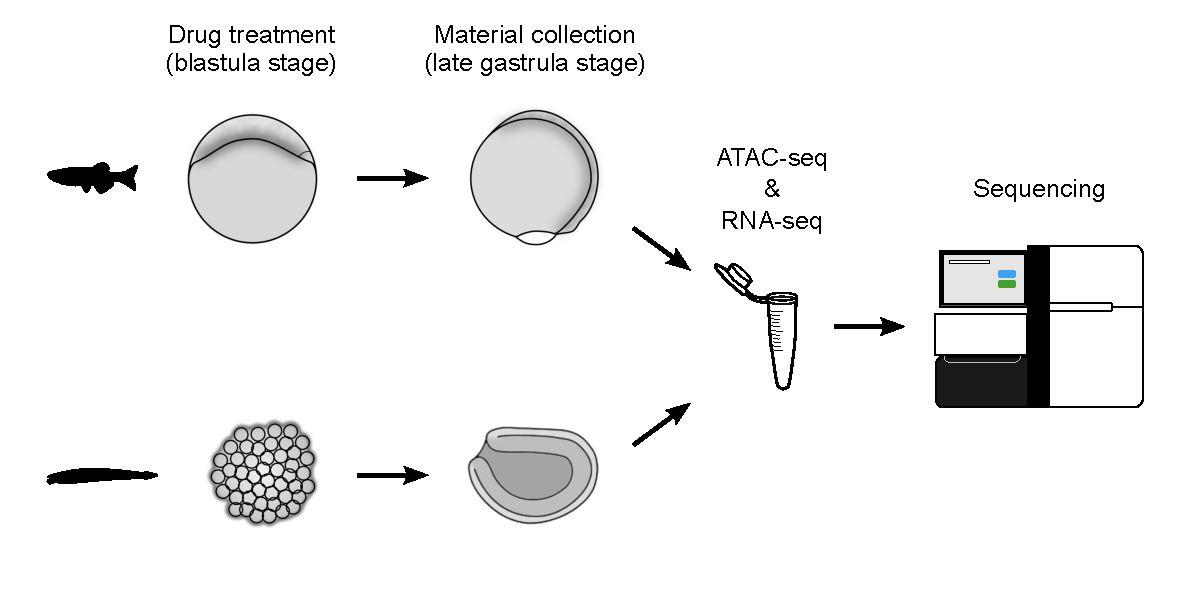
\includegraphics[width=1\textwidth]{Figures/squeme_drug_treatment}
\caption[Drug treatment scheme]{ Experimental design of signalling pathways disruption. Zebrafish and amphioxus embryos were treated from the late-blastula developmental stage until they developed into the late-gastrula stage. The embryos at the late-gastrula stage were collected and dissociated in order to generate next-generation sequencing libraries for ATAC-seq and RNA-seq. Modified from \parencite{gil-galvez_gain_2022}.
}
\label{fig:drug_squeme}
\end{figure} 




 To assess the consequences of the altered signalling pathways in gene regulation, we generated and analysed transcriptomic (RNA-seq) and epigenetic (ATAC-seq) data from treated and control embryos at the gastrula stage. First, by comparing gene expression of treated versus control embryos, we found at least hundreds of genes transcriptomically affected for each treatment (Figure \ref{fig:MA_plots}). Due to their expression change, these genes were considered to be under the control of the treated signalling pathways during development. To get a general insight into the functions of these genes, we performed Gene Ontology (GO) enrichment analysis, in which each of them is associated with the general categories of  Metabolism, Development and Others. Indeed, some of the most differentially expressed genes were effector genes of the altered signalling pathways and the processes that they have associated, validating the efficacy of the drug treatments (Figure \ref{fig:effect_of_treatments}). We found that the number of affected genes associated with developmental terms was greater in zebrafish than in amphioxus.
 
Next, in order to investigate the evolutionary differences in gene regulation between amphioxus and zebrafish, we set out to compare the transcriptomic data sets from both species. Since amphioxus has not undergone the vertebrate and the teleost WGDs, we could not compare genes in a 1-to-1 manner. To address this problem, we worked with gene families (orthogroups) previously computed in \parencite{marletaz_amphioxus_2018}. These orthogroups are considered the ohnolog families between zebrafish and amphioxus. Whenever we had to search for orthologs genes of amphioxus genes, we used these orthogroups in the following manner. For each gene of amphioxus, we identify the orthogroup it belonged to. From that orthogroup, we retrieve all the zebrafish genes that are orthologous to the amphioxus gene since they belong to the same orthogroup. Due to the lack of functional annotation in amphioxus genes, we had to perform GO enrichment of amphioxus genes using the GO databases of zebrafish, using the orthologous genes. We compared the downstream transcriptomic response of genes induced by the same treatment in both species, and we found that the lists of differential genes in both species were generally overlapping. We found a large overlap of affected genes in amphioxus, while their orthologs in zebrafish were also altered. We conducted GO enrichment of the commonly affected genes in order to reveal which is the function of these genes (Figure \ref{fig:common_affected_genes}). Interestingly, there was little overlap of genes when analysing the effect of Wnt agonist treatment in both species. The functions of these commonly affected genes were expected since they affect developmental tissues regulated by these signalling pathways \parencite{bertrand_developmental_2017, kiecker_molecular_2016, tuazon_temporally_2015}.


\begin{figure}[hp]
\centering
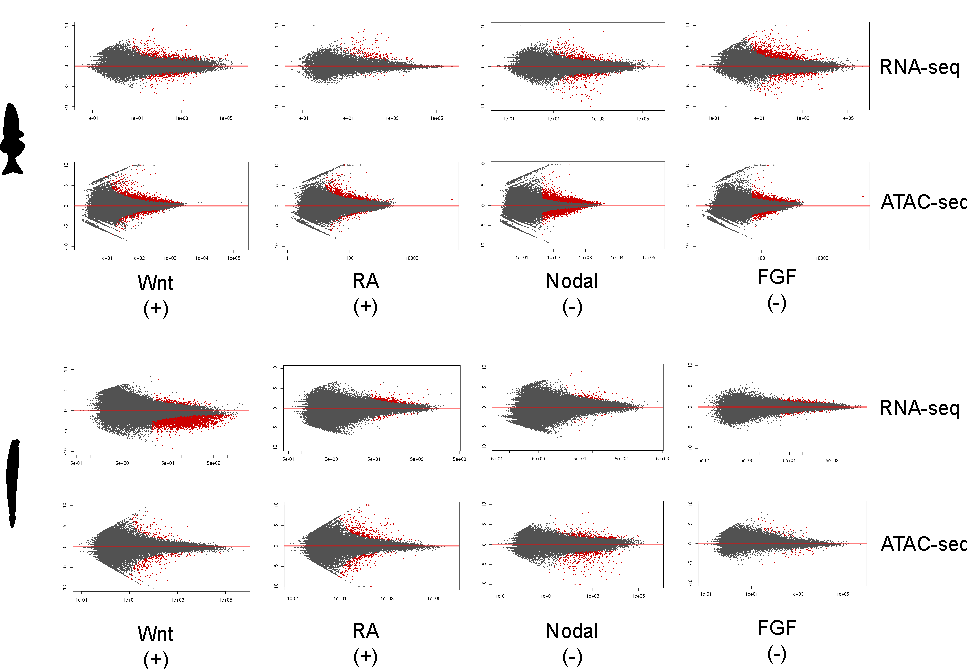
\includegraphics[width=1\textwidth]{Figures/MA_plots}
\caption[MA plots]{ Effect of the different treatments in both species at transcriptomic and epigenomic levels. Each dot is a gene in RNA-seq plots and a peak in ATAC-seq plots. Genes or peaks that are significantly different between the treatment and control conditions are represented in red. On the X axis is represented the expression/aperture levels and in the Y axis the log2(Fold change). Modified from \parencite{gil-galvez_gain_2022}.
}
\label{fig:MA_plots}
\end{figure} 

\begin{figure}[hp]
\centering
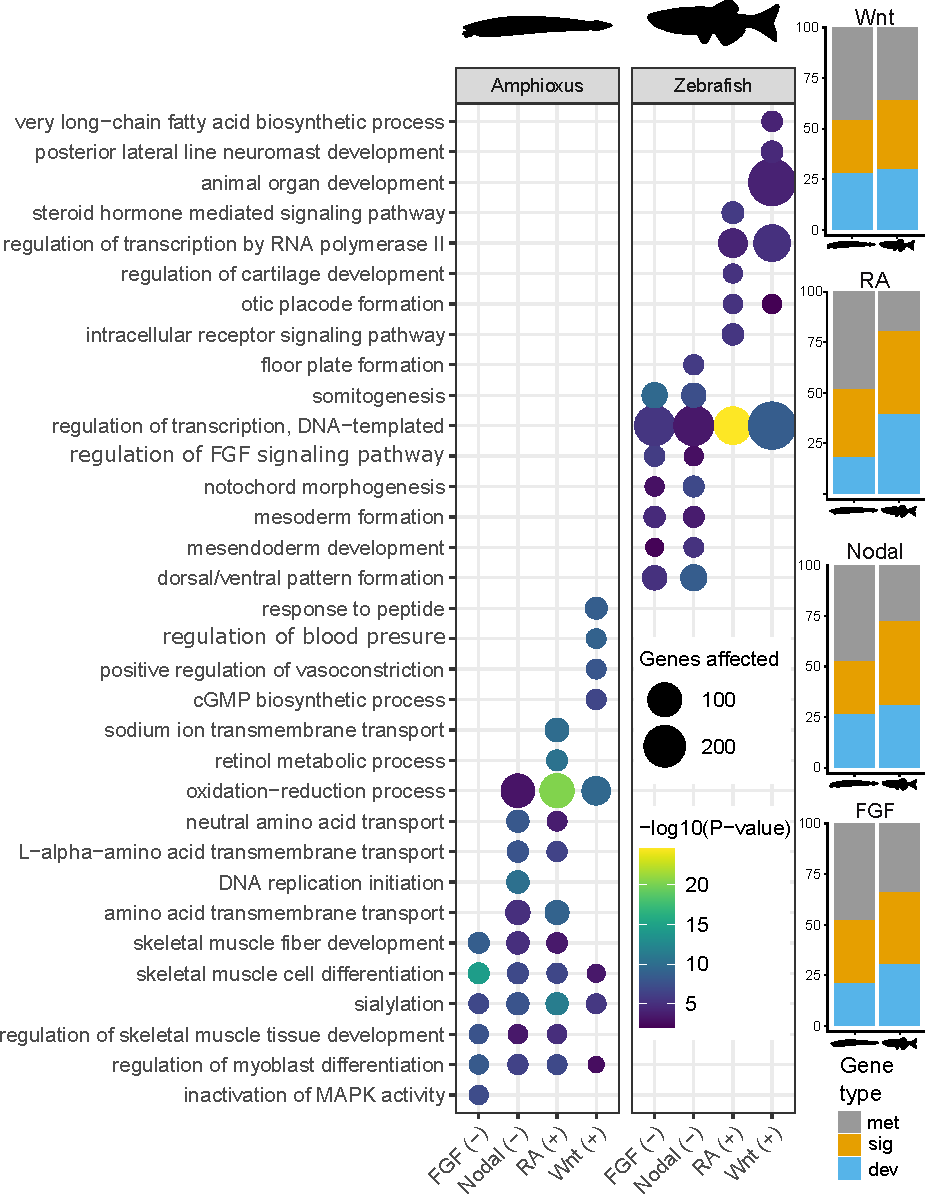
\includegraphics[width=1\textwidth]{Figures/Effect_of_treatments_GOs_v2}
\caption[Transcriptomic effects of the treatments]{ Gene Ontology and gene types of the genes affected by the treatments. The X-axis represents each drug treatment, with amphioxus on the left panel and zebrafish on the right one. The Y-axis represents the enriched GO terms. The dot size is proportional to the number of genes enriched in the corresponding GO term. The colour of the dots varies with the $-log10(PValue)$ of the enrichment. On the right, the proportion of gene types is represented by bar plots. Each treatment is represented, and the type of gene that they affect in each species. Grey colour indicates metabolic genes, orange colour indicates signalling genes and blue colour denotes developmental genes. Modified from \parencite{gil-galvez_gain_2022}.
}
\label{fig:effect_of_treatments}
\end{figure} 


\begin{figure}[h]
\centering
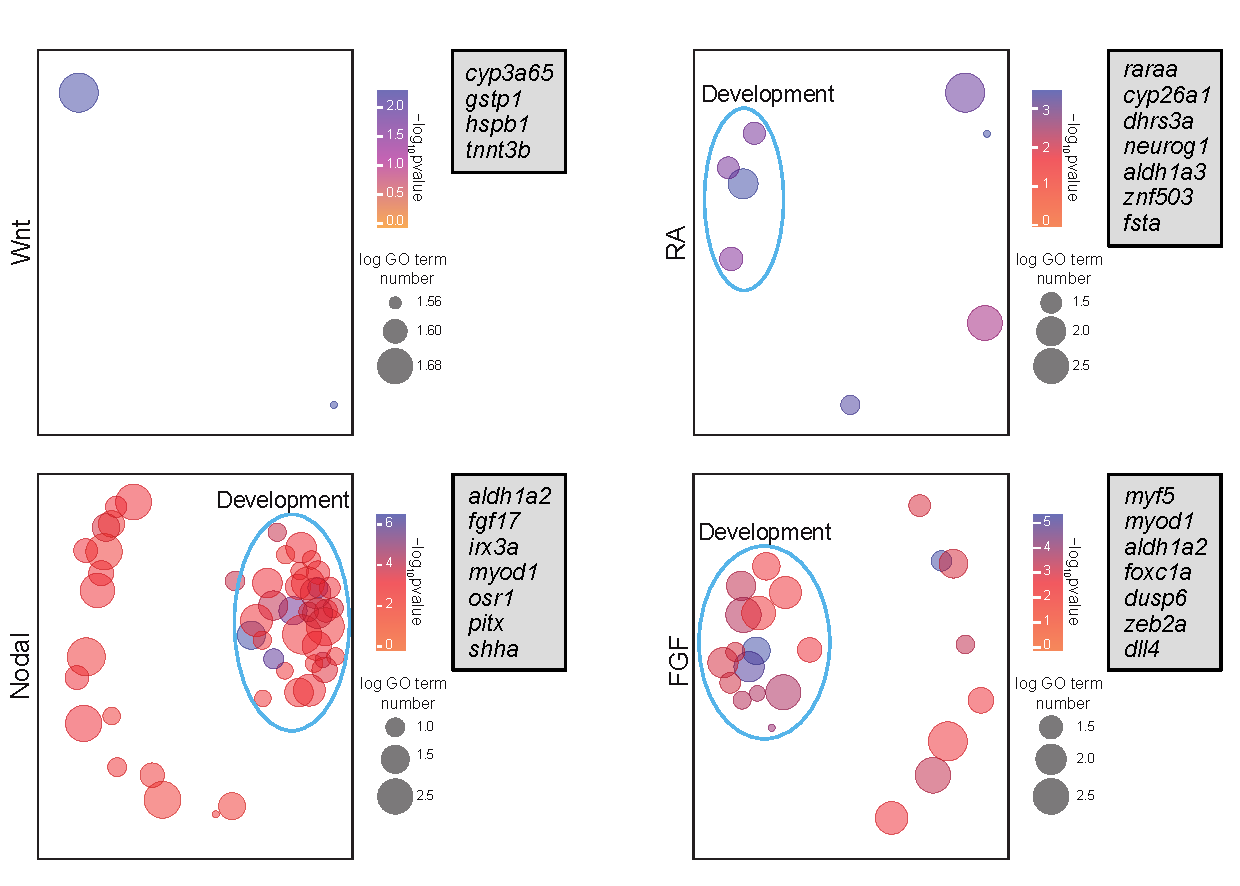
\includegraphics[width=1\textwidth]{Figures/fib1b_GO_common_orthologs}
\caption[GO term enrichment of the commonly affected orthologs]{
GO enrichment for the orthologs affected by the same treatment in both species. Each dot represents GO terms and dots are distributed in an X-Y semantic space. GOs that are more similar cluster together. Developmental GOs are encircled with a blue line.  Modified from \parencite{gil-galvez_gain_2022}.
}
\label{fig:common_affected_genes}
\end{figure} 


\begin{figure}[hp!]
\centering
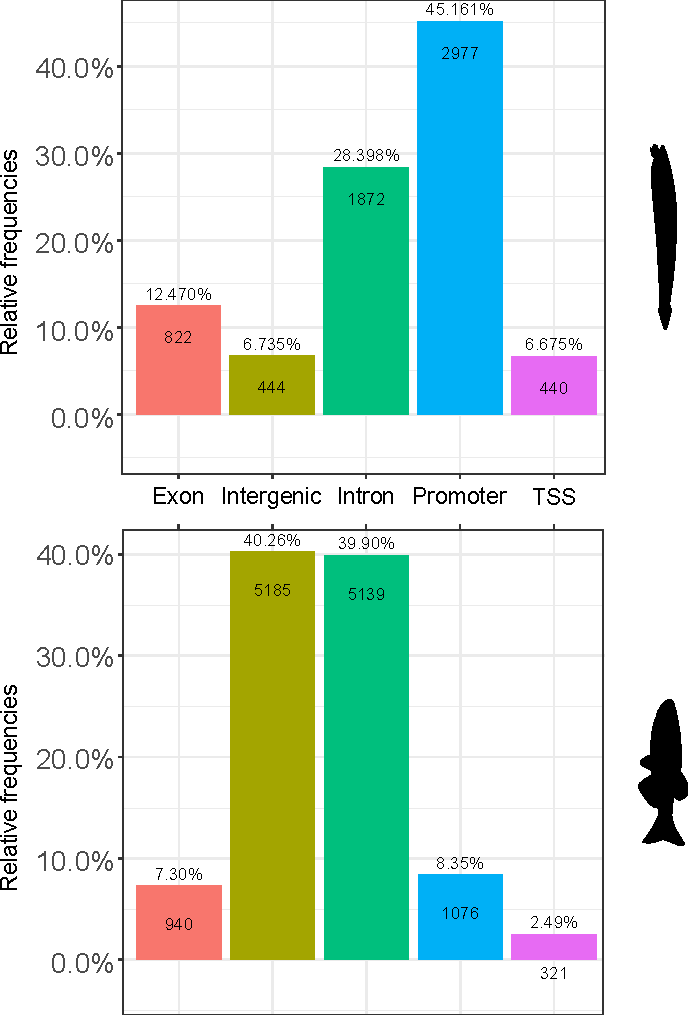
\includegraphics{Figures/Distribution_DARs}
\caption[Genomic distribution of DARs]{ Distribution of genomic positions of DARs in zebrafish and amphioxus. Promoter regions are defined by -1kb to +100bp from the TSS of the neighbour gene. TSS region is defined by -100bp to +1kb from the TSS. Modified from \parencite{gil-galvez_gain_2022}
}
\label{fig:distribution_DARS}
\end{figure} 

In order to know which CREs were changing their accessibility status upon treatment, we performed differential analysis on our ATAC-seq data in both species. We detected the open chromatin regions across conditions and then addressed if there was differential accessibility between treated and control conditions using DESeq2 \parencite{love_moderated_2014}. Using this strategy, we found several hundreds of differentially accessible regions (DARs, Figure \ref{fig:MA_plots}). First, we assessed how these DARs distribute in the genome of zebrafish and amphioxus. We found that, compared to zebrafish, in amphioxus, they tend to be more proximal to the target gene (Figure \ref{fig:distribution_DARS}). In accordance with previous work from the lab, \parencite{marletaz_amphioxus_2018}, in zebrafish, most of the DARs were placed in intergenic regions (39.9\%) and intronic regions (40.26\%), and the rest of the DARs were located in the promoter region (8.35\%) or exonic regions (7.3\%). In zebrafish, there was a 1.36\% of DARs which location could not be determined properly.  In contrast, most DARs detected in amphioxus were located in promoter regions (45.16\%), with a small proportion of them located in intergenic regions (6.74\%). The rest of amphioxus DARs were located in exon regions (12.47\%), intronic regions (28.398\%) or TSS regions (6.675\%). In amphioxus, there was a 0.5\% of DARs which could not be assigned. To investigate which TFs operate on these DARs, we performed TFBS enrichment analysis (Figure \ref{fig:ATAC_motifs_pathways}). In detail, we computed which TFs have their TFBS overrepresented in each dataset of DARs sequences compared to the entire set of ATAC-seq regions. As a result, we found that, regardless of the genomic distribution, these DARs were bound by TFs that are known effectors of the altered signalling pathways \parencite{bottcher_fibroblast_2005, cadigan_tcflefs_2012, charney_gene_2017, bian_clock1a_2017, jia_smad2_2008, kjolby_integration_2019,tian_nodal_2006, friedman_foxa_2006, ghyselinck_retinoic_2019, hoodless_foxh1_2001, joshi_cdx4_2019, kjolby_genome-wide_2017, aldea_genetic_2019, onai_canonical_2019, yasuoka_evolution_2019}. For example, in both species, we found that, upon RA treatment, the set of detected DARs is enriched in RAR:RXR TFBS, as they are the direct effectors of this pathway \parencite{ghyselinck_retinoic_2019}. Moreover, we could detect not only the direct effectors of the affected signalling pathways but also the secondary effectors of these pathways in both species. For example, we observed an enrichment of \textit{tcf} TFBS in both species upon agonist treatment of Wnt signalling pathway \parencite{cadigan_tcflefs_2012,kjolby_genome-wide_2017,kjolby_integration_2019}. Taken together, these results confirm that the drug treatments against specific signalling pathways alter the gene expression of effectors involved in those pathways and the relevant developmental processes.

\begin{figure}[hp]
\centering
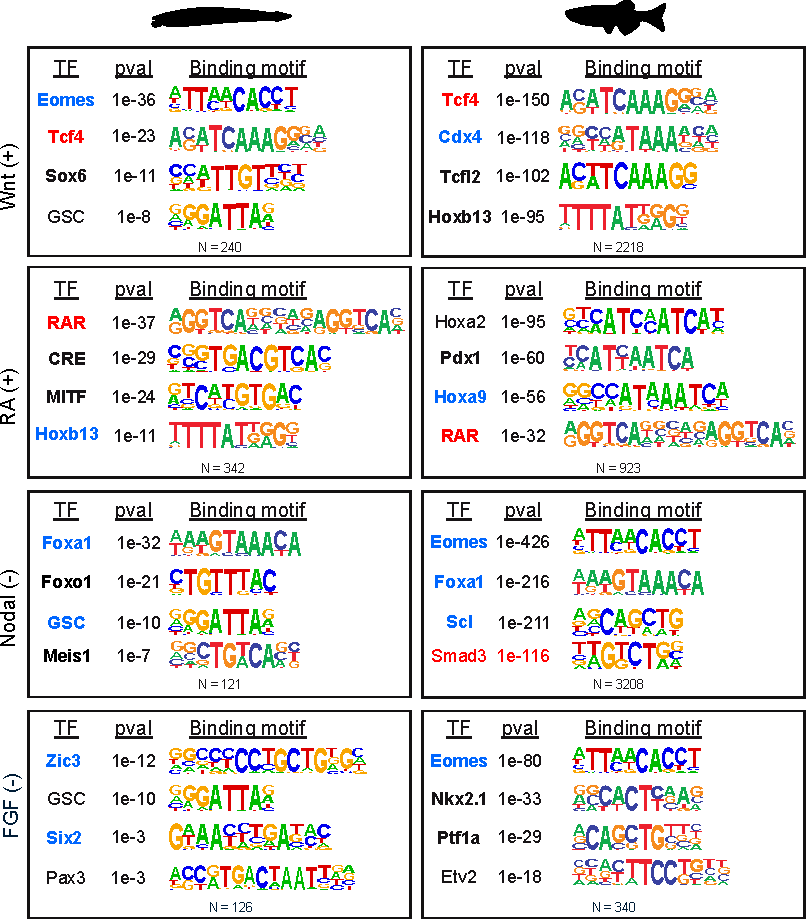
\includegraphics[width=1\textwidth]{Figures/ATAC_motif_pathways}
\caption[Motif enrichment of DARs]{ Motif enrichment analysis of DARs for each treatment and species. Only the four most relevant TFBS are shown. Names of the relevant TFs, enrichment p-values and binding motifs  are shown in each box. At the bottom of each box is the number of DARs for the corresponding species and treatment. Downstream effectors of the signalling pathways are represented in blue. Direct effectors of the altered pathway are shown in red. TFs whose motifs are enriched in both species are represented in bold font. Modified from \parencite{gil-galvez_gain_2022}.
}
\label{fig:ATAC_motifs_pathways}
\end{figure} 

Upon confirming the direct effect of the altered signalling pathways on regulatory regions of the genome, we aimed to assess the developmental role of those regions. Although we could observe the binding of known effector TFs of the pathways on these DARs, we wondered at which developmental stages these DARs were active, and whether we were modifying that timing. First, we intersected our CREs with the developmental CREs that were studied in the work of Marletaz and colleagues \parencite{marletaz_amphioxus_2018}, and we found that our CREs were a subset of the developmental CREs in both species. Secondly, we wanted to address how dynamic the chromatin was during the development in our CREs. To do that, we used previously published ATAC-seq data in both species \parencite{marletaz_amphioxus_2018}, including different developmental stages of zebrafish and amphioxus. We examined the signal of our DARs in this dataset for each species, and we found that most DARs that arose upon treatments were indeed dynamic regions during development in both species (Figure \ref{fig:Dynamic_behaviour}). This analysis revealed that the treatments made these DARs active at different developmental stages than in a WT situation. For example, in the RA treatment in both species, we observe groups of DARs in which normal opening occurs at late stages. Our treatment led to the opening of these regions before, at 80\% of epiboly.



\begin{figure}[hp]
\centering
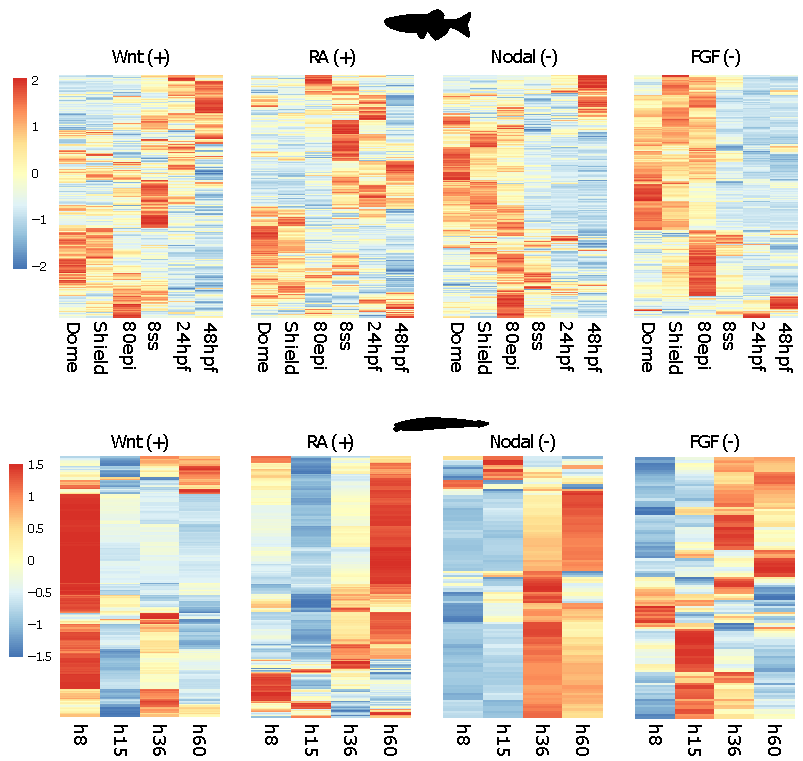
\includegraphics[width=1\textwidth]{Figures/Dynamic_behaviour}
\caption[DARs developmental dynamics]{ Dynamics of ATAC-seq signal during development in DARs detected in the treatments. For each species and treatment, the corresponding DARs are examined, and the ATAC-seq signal during developmental stages is represented. The panel within each species analysis represents heatmaps which demonstrate the dynamics of groups of DARs for each treatment during development. The selected developmental stages in zebrafish are Dome, dome stage; Shield, shield stage; 80epi, 80\% of epiboly; 8ss, 8 somites; 24hpf, 24 hours post fertilization (hpf); 48hpf. The selected stages for amphioxus are: h8, 8 hpf, corresponding to early gastrula stage (G3); h15, 15 hpf, corresponding to early neurula stage (G6); h36, 36 hpf, corresponding to premouth stage (T0); h60, 60 hpf, corresponding to early larvae stage (L0-L1). Modified from \parencite{gil-galvez_gain_2022}.
}
\label{fig:Dynamic_behaviour}
\end{figure} 

Once we addressed the ATAC-seq and RNA-seq individually for each treatment, we wanted to study patterns of gene expression or chromatin opening. In order to do so, we performed clustering analysis of RNA-seq and ATAC-seq separately, grouping genes or DARs according to their response to the different treatments. To identify patterns of transcriptomic behaviour across the different treatments, we classified the affected genes of both species by clustering their RNA-seq signal (Figure \ref{fig:RNAseq_clustering}). The resulting clusters represent groups of genes which have a similar transcriptional pattern. We then explored the functions of the resulting gene clusters using GO enrichment analyses. We found that in zebrafish, these gene clusters have development-related functions. In amphioxus clusters, genes also show developmental functions, but we could also find enrichment in terms related to metabolism and non-developmental processes are also enriched. This result aligns with the previous finding (Figure \ref{fig:effect_of_treatments}) since in amphioxus, responsive genes were more related to non-developmental functions. There were several examples of how these clusters represented genes with similar transcriptional responses to the treatments. For example, the induced-by-RA gene clusters in both species (dark blue in amphioxus and light orange in zebrafish) associate with GO terms related to the RA pathway, such as retinol metabolism and central nervous system development. Similarly, the orange cluster of amphioxus is associated with Nodal downregulated genes and is related to mesodermal developmental terms such as muscle development. Additionally, we have found some GO terms enriched in more than one gene cluster, meaning that different signalling pathways affect the same process.  For instance, somitogenesis appears to be affected in zebrafish in light-blue (FGF-associated) and dark orange (Wnt and Nodal) clusters. In summary, clustering of the differentially expressed genes upon treatment shows that in zebrafish the GO terms are more related to developmental processes than in amphioxus and, more importantly, that some biological functions are affected by two or more signalling pathways in both species.



\begin{figure}[hp]
\centering
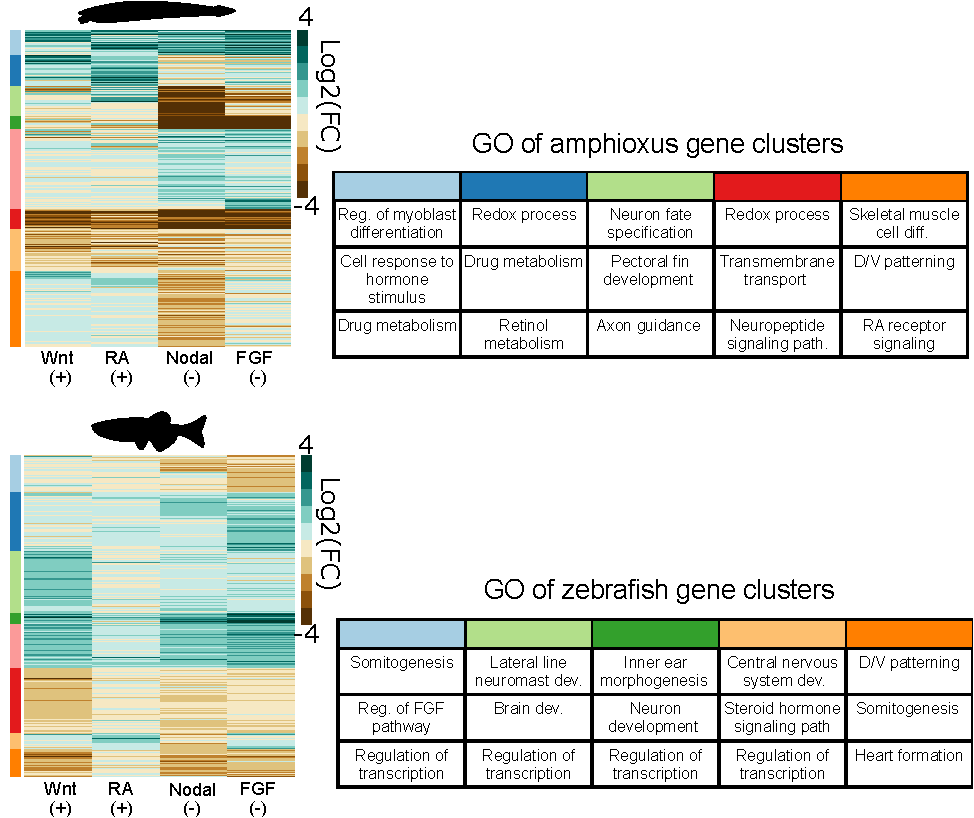
\includegraphics[width=1\textwidth]{Figures/RNA_seq_clustering_v2}
\caption[Transcriptomic clustering of the responsive genes to treatments in both species]{Transcriptomic clustering of responsive genes to treatments in both species (top: amphioxus, bottom: zebrafish) based on RNA-seq log2 Fold Change (Log2FC). Genes were clustered based on their FC similarity across conditions. On the right, selected GOs enriched in the corresponding cluster are represented. In these tables, only selected GO terms from gene clusters with clear patterns of expression are represented. Modified from \parencite{gil-galvez_gain_2022}.
}
\label{fig:RNAseq_clustering}
\end{figure} 

We also applied clustering analysis to the ATAC-seq signal to assess how complex were the regulatory changes and to further discern DARs according to their response. In order to associate the potential enhancers with their target genes, we used the GREAT algorithm \parencite{mclean_great_2010}, which associates DARs with closeby genes. Next, we computed GO enrichment analyses for all the genes affected in each cluster. Similarly to previous results, we found several functions related to the corresponding altered signalling pathway that was being treated in each of the clusters. Furthermore, we computed TFBS enrichment for each cluster, finding the binding site of some of the effector TFs of the pathways (Figure \ref{fig:ATACseq_clustering}). For example, in zebrafish, the blue cluster included Wnt responsive elements and the GO terms enriched for that cluster were related to brain development. Moreover, inside these ATAC regions, the TFBS of a known Wnt-related effector, \textit{TCF3}, was enriched \parencite{cadigan_tcflefs_2012, kjolby_genome-wide_2017}. We observed similar results in the cluster of regions that were controlled by RA in both species (dark green cluster in zebrafish and dark purple in amphioxus). Both clusters presented an enrichment in known functions of RA, like hindbrain development, and in the RAR:RXR motif. It is important to note that the mentioned cluster in zebrafish was also responding to Wnt treatment. To obtain a quantitative measure of the similarity of these clusters, we used the GO terms enriched in each cluster and computed the GO similarity scores between the zebrafish and amphioxus clusters (Figure \ref{fig:ATAC_go_similar}). We observed that clusters of ATAC-seq peaks that respond to the same treatment tended to have higher similarity scores, as in the case of the aforementioned RA clusters. Conversely, there were some clusters with very low scores of similarity, like the Nodal cluster of amphioxus (blue), and any of the zebrafish ones. 




\begin{figure}[hp]
\centering
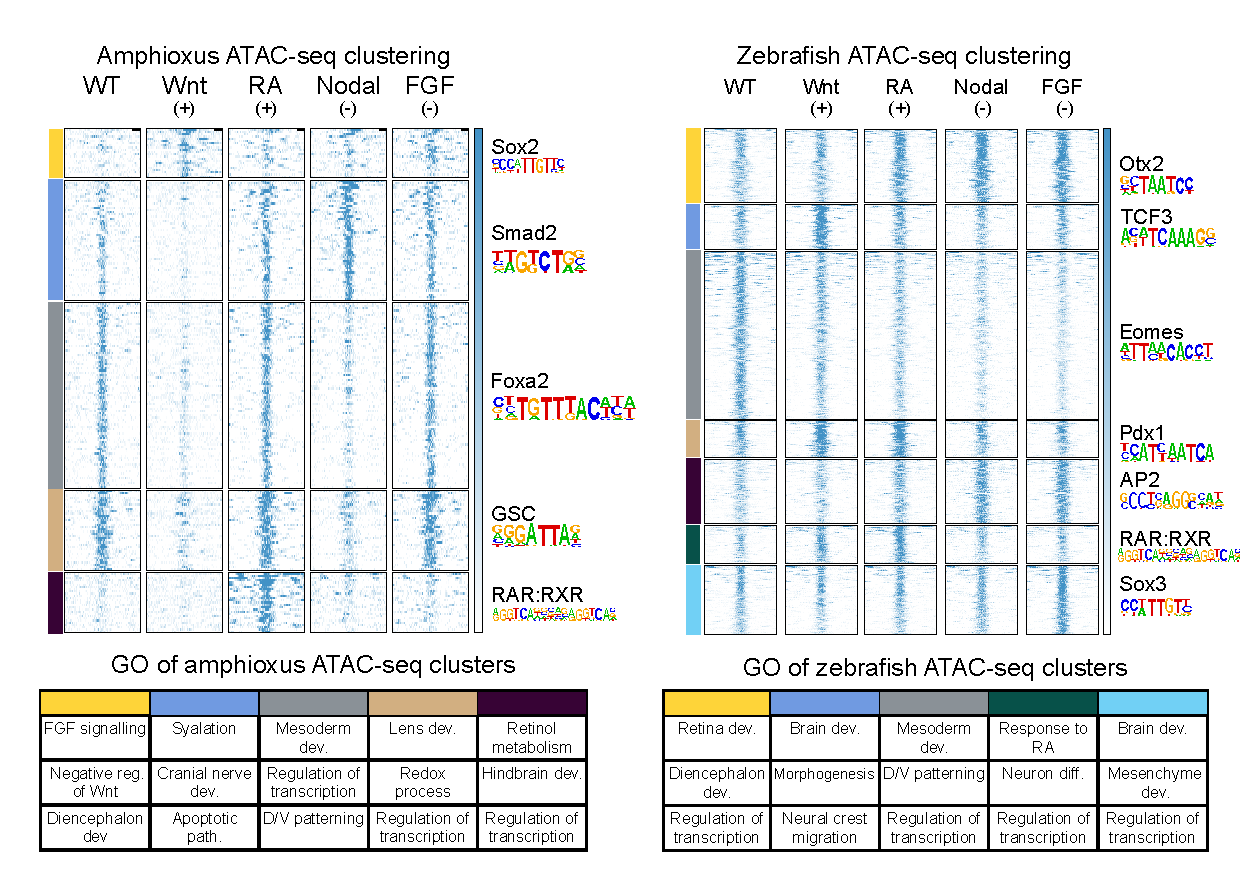
\includegraphics[width=1\textwidth]{Figures/ATACseq_clustering.pdf}
\caption[ATAC-seq clustering of open chromatin regions]{ATAC-seq clustering of open chromatin regions in amphioxus (left) and zebrafish (right). The most enriched TFBS found in each cluster is represented on the right. Below is a selection of important enriched GO terms for clusters with clear patterns of chromatin aperture. Modified from \parencite{gil-galvez_gain_2022}. 
}
\label{fig:ATACseq_clustering}
\end{figure} 

\begin{figure}[hp]
\centering
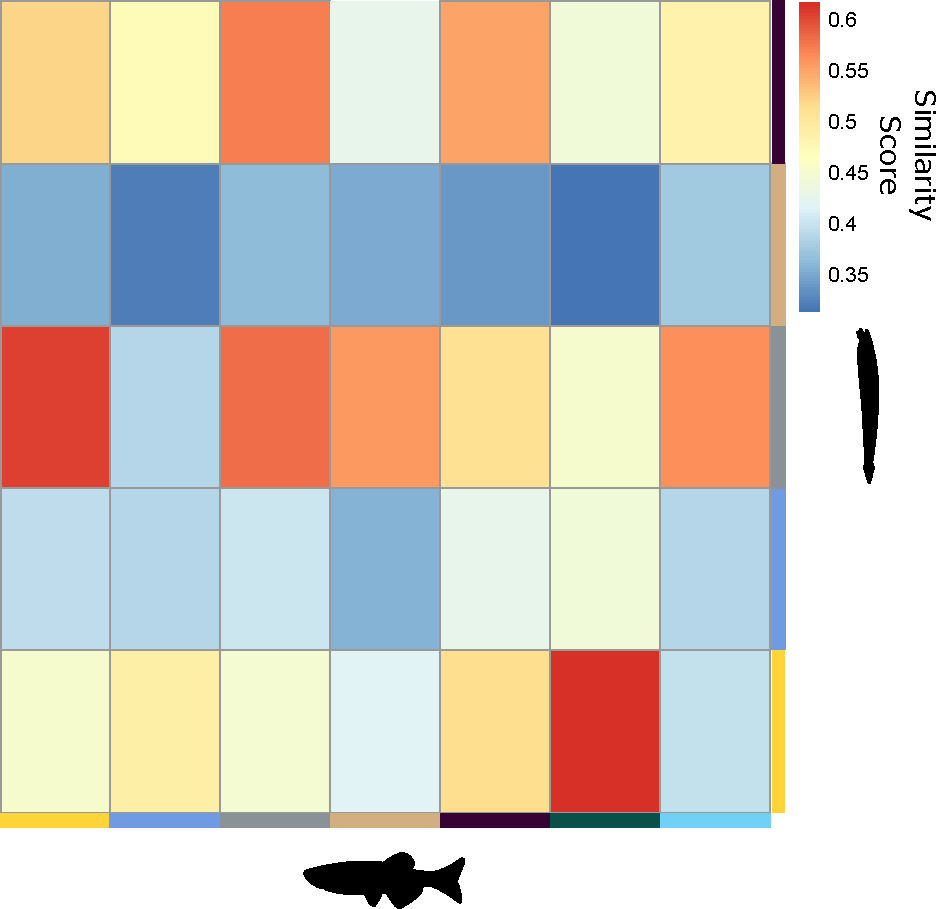
\includegraphics[width=1\textwidth]{Figures/ATAC_go_similar}
\caption[Similarity of ATAC-seq clusters based on GO terms]{
Similarity scores of ATAC-seq clusters based on GO terms. Heatmap representing pairwise GO similarity scores for each cluster in both species. Each cluster maintains the same colour scheme as in (Figure \ref{fig:ATACseq_clustering}). Modified from \parencite{gil-galvez_gain_2022}.
}
\label{fig:ATAC_go_similar}
\end{figure} 

\newpage

\section{Gain of GRN connectivity during vertebrate evolution}
\label{sec:Interconnectivity_chatper_sub2}

During the clustering analysis of RNA-seq (Figure \ref{fig:RNAseq_clustering}) and ATAC-seq (Figure \ref{fig:ATACseq_clustering}), we observed that some groups of genes and DARs were responding to more than one treatment, like the ATAC-seq RA cluster. This means that some genes and CREs are under the regulatory control of more than one signalling pathway in both species. We computed connectivity scores for each DAR, which range from 1 to 4, depending on the number of treatments to which they responded (Figure \ref{fig:ATAC_connectivity}). In comparison to amphioxus, zebrafish had DARs with higher connectivity score in average, meaning that the number of DARs responding to more than one signalling pathway is greater. Also, in amphioxus, only 16 DARs presented a connectivity score of 3, and no DARs were affected by all the four treatments, whereas the number of DARs with connectivities of 3 and 4 in zebrafish was 501 and 137, respectively. 
We next assessed the connectivity among the different signalling pathways. To do this, we computed the overlap of responsive DARs (upregulated or downregulated) between the different treatments (Figure \ref{fig:ATAC_connectivity}). We first observed that, although the degree of overlap was greater in zebrafish, there was a high level of variation in both species. In amphioxus, the overlap ranged from 0 to 72.4\%, whereas in zebrafish, this range increased from 0 to 89.1\%. Interestingly, the clusters sharing the highest overlap in both species were not the same. In amphioxus, the highest overlap was found between the group of DARs that were downregulated upon RA treatment and the Wnt downregulated ones. Still, in zebrafish, it was between the downregulated in Nodal and downregulated in FGF.
 
 
\begin{figure}[hp]
\centering
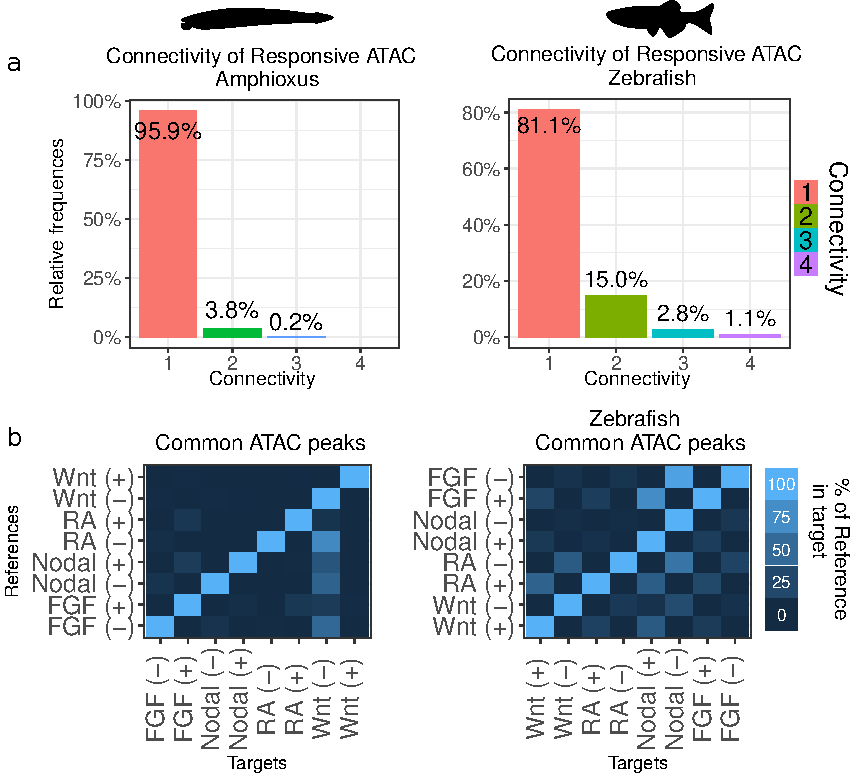
\includegraphics[width=1\textwidth]{Figures/ATAC_connectivity}
\caption[Connectivity of DARs in both species]{ Degree of connectivity of DARs in both species. \textbf{a} Barplots representing the frequencies of peaks that are responding to one, two, three or four treatments in amphioxus (left) and zebrafish (right). \textbf{b} Heatmaps showing the percentages of overlap between DARs of different conditions. Modified from \parencite{gil-galvez_gain_2022}.
}
\label{fig:ATAC_connectivity}
\end{figure} 



In order to identify core genes that may drive the response to treatments, we integrated these data at the gene level, selecting genes detected by ATAC that responded by being targets of a nearby DAR and which RNA-seq signal changed upon the treatment. In this study, we named these genes double-selected genes (DSG). This integration was performed without considering whether the treatments were inhibitory or activating in order to get the total of core DSGs. We determined the correlation of ATAC-seq and RNA-seq signals in these DSGs, in order to have a better understanding of their regulation, and we could find only a mild correlation (Figure \ref{fig:DSG_ATAC_RNA_correlation}). Only when categorizing the expression levels and accessibility levels in three different categories (low, medium and high, based on the normalized signal of each feature) we found a correlation between the ATAC and RNA-seq signal in DSGs. DSGs categorized as lowly expressed tended to have associated DARs with less opening than the others.  This underlines that ATAC-seq and RNA-seq do not always correlate in signal, but they can still reflect the underlying genomic regulation of the target gene. 
In total, we selected 2098 DSGs associated with 4609 DARs in zebrafish and 481 DSGs associated with 853 DARs in amphioxus, a difference that indicates a gain in regulatory input during the chordate-to-vertebrate transition. The incorporation of new CREs is a likely explanation for the increased responsiveness of the studied signalling pathways. Next, to dive into the functions of these DSGs, we performed GO enrichment in each set of DSGs responding to the treatments (Figure \ref{fig:DGS_GOs_pval}). We demonstrated that a higher number of GO terms are enriched in two or more signalling pathways in zebrafish than in amphioxus. This agrees with the fact that, in zebrafish, more DSGs responded to signalling pathway disruption than in amphioxus. 
In summary, not only the number of responsive genes is different between the two species, but also the variability of functions, suggesting that vertebrates built more complex developmental networks during the transition from invertebrate chordates.



 
\begin{figure}[hp]
\centering
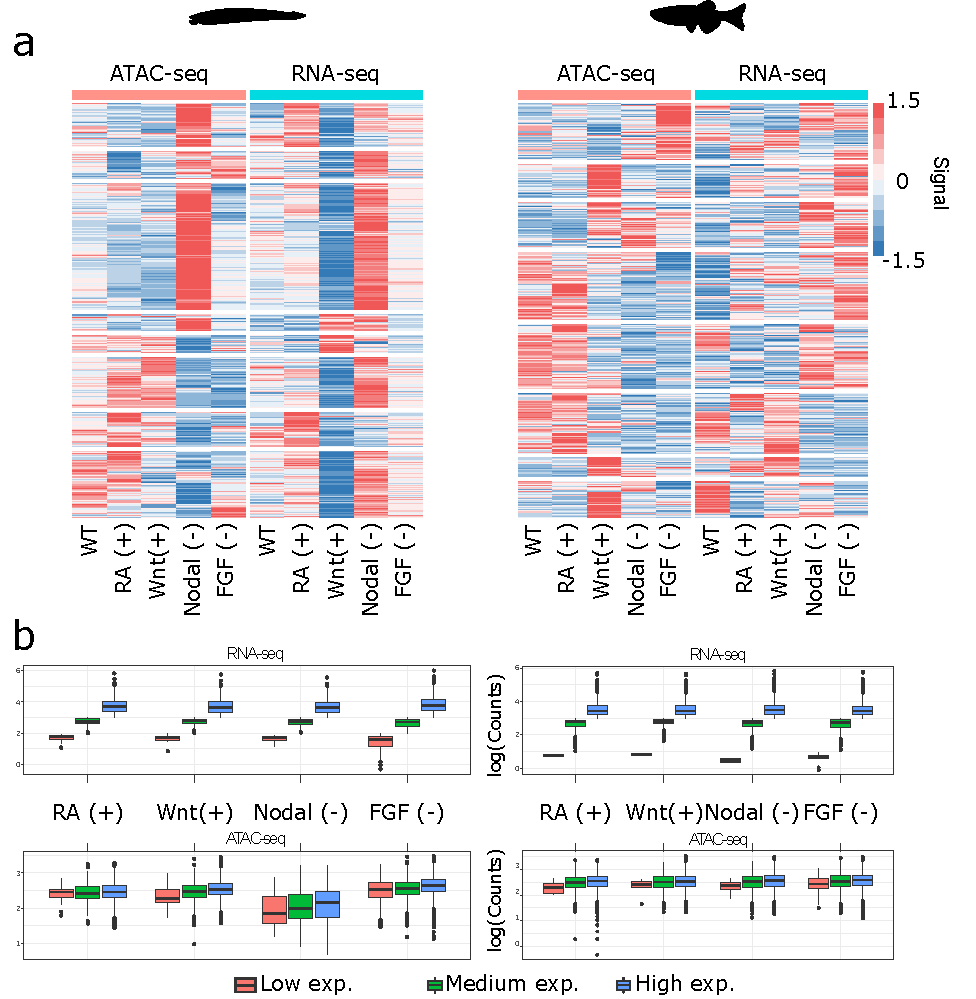
\includegraphics[width=1\textwidth]{Figures/DSG_ATAC_RNA_correlation}
\caption[Correlation of DSGs]{Correlation of DSG signal at ATAC-seq and RNA-seq level. The correlation is computed based on the ATAC-seq signal of the peaks overlapping the promoter of a gene and the RNA-seq signal of the gene. \textbf{a} Heatmap representing ATAC-seq and RNA-seq signal for each gene. \textbf{b} Distribution of ATAC-seq and RNA-seq signals for genes subdivided into three different groups based on their expression level. Modified from \parencite{gil-galvez_gain_2022}.

}
\label{fig:DSG_ATAC_RNA_correlation}



\end{figure} 
 
\begin{figure}[hp]
\centering
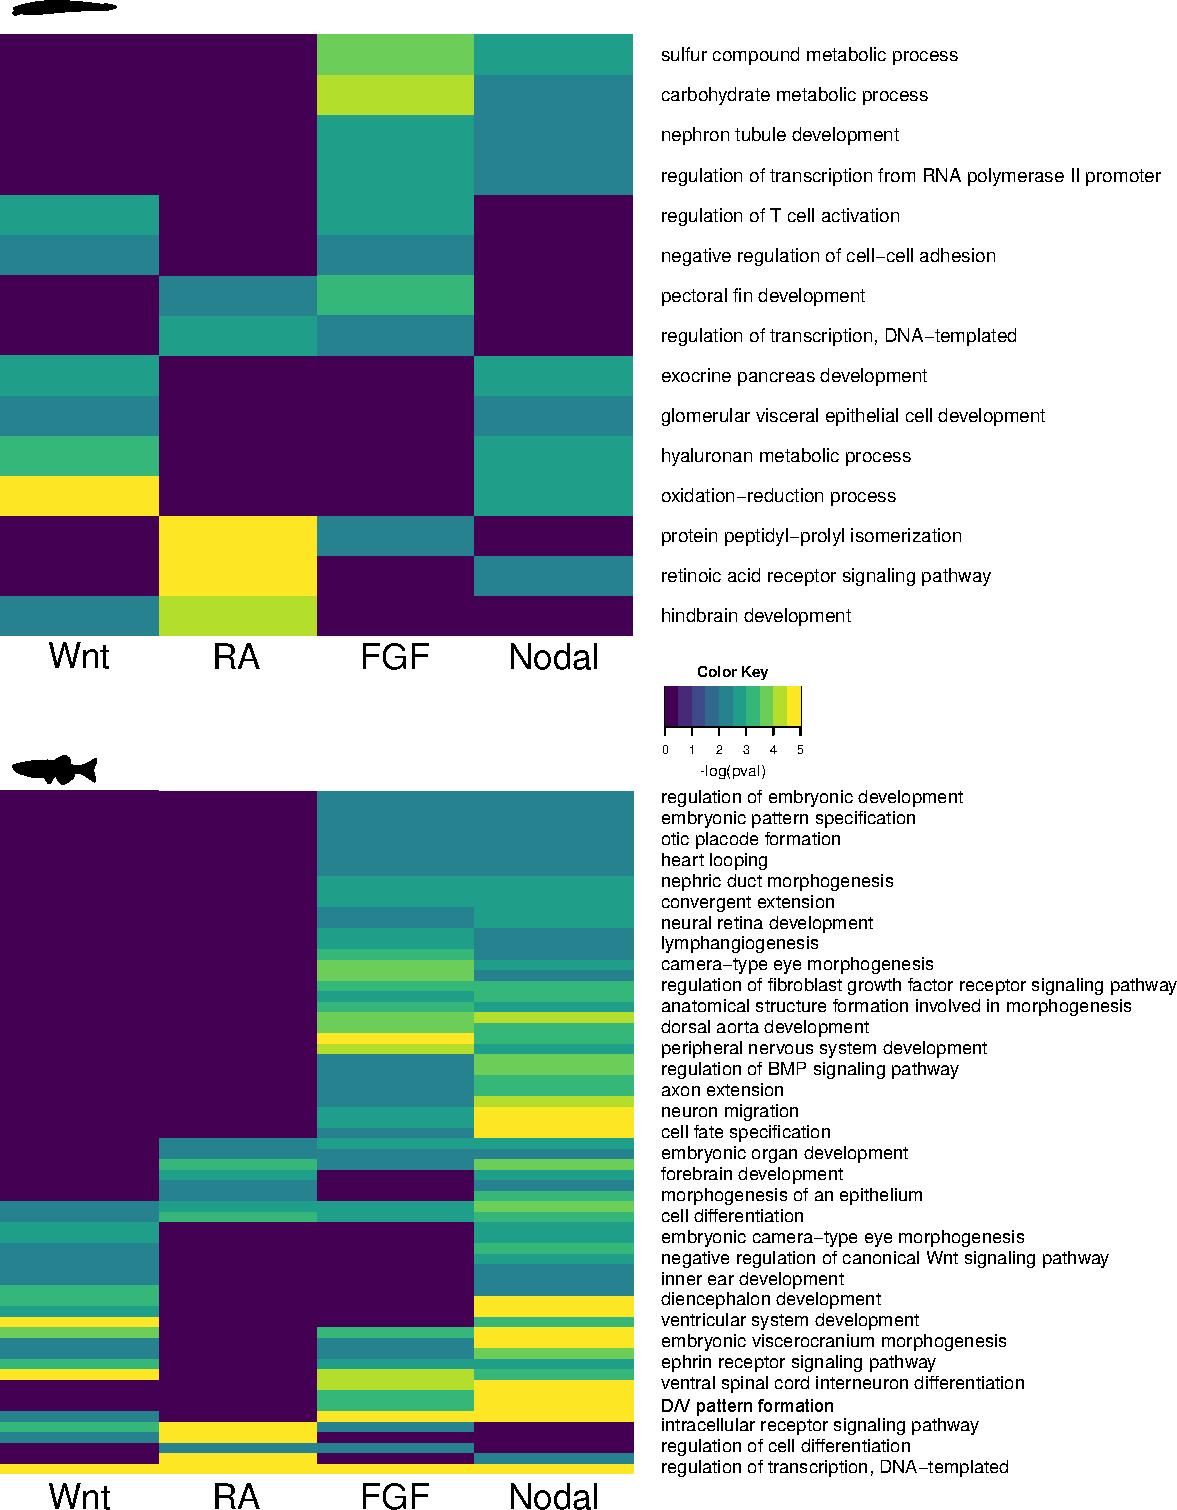
\includegraphics[width=1\textwidth]{Figures/DSG_GOs_pval}
\caption[GO enrichment clustering of DSGs in both species]{GO enrichment clustering of DSGs in both species. The heatmaps show how the different GO terms are clustering based on the -log10(p-value) in amphioxus (top) and in zebrafish (bottom). Modified from \parencite{gil-galvez_gain_2022}.
}
\label{fig:DGS_GOs_pval}
\end{figure} 

However, for each amphioxus DSG, we included all zebrafish ortholog genes in order to compute GO enrichment, probably inflating the GO enrichment \textit{P}value in zebrafish. To avoid this potential bias, we analysed the GO enrichment of amphioxus DSGs using the entire orthology group of these DSGs in zebrafish. Here, for each enriched GO term, we represented how many gene families of DSGs were affected upon treatments (Figure \ref{fig:DGS_GOs_fams}). Interestingly, this approach revealed greater differences between zebrafish and amphioxus. We found that some functions had low \textit{P}values in amphioxus. But when exploring the number of gene families responsible for that function, we found few of them in amphioxus. This was the case for example in hindbrain development GO term in amphioxus. In addition, in zebrafish, more families of genes responded to these functions than in amphioxus, reinforcing the idea that there was a gain of regulatory information in the former. Moreover, in zebrafish, we found more GOs related to the signalling pathways and development, such as the Wnt signalling pathway. Together, these results suggest an increase in the number of genes controlled by the treated signalling pathways in zebrafish.

 
 
 
\begin{figure}[hp]
\centering
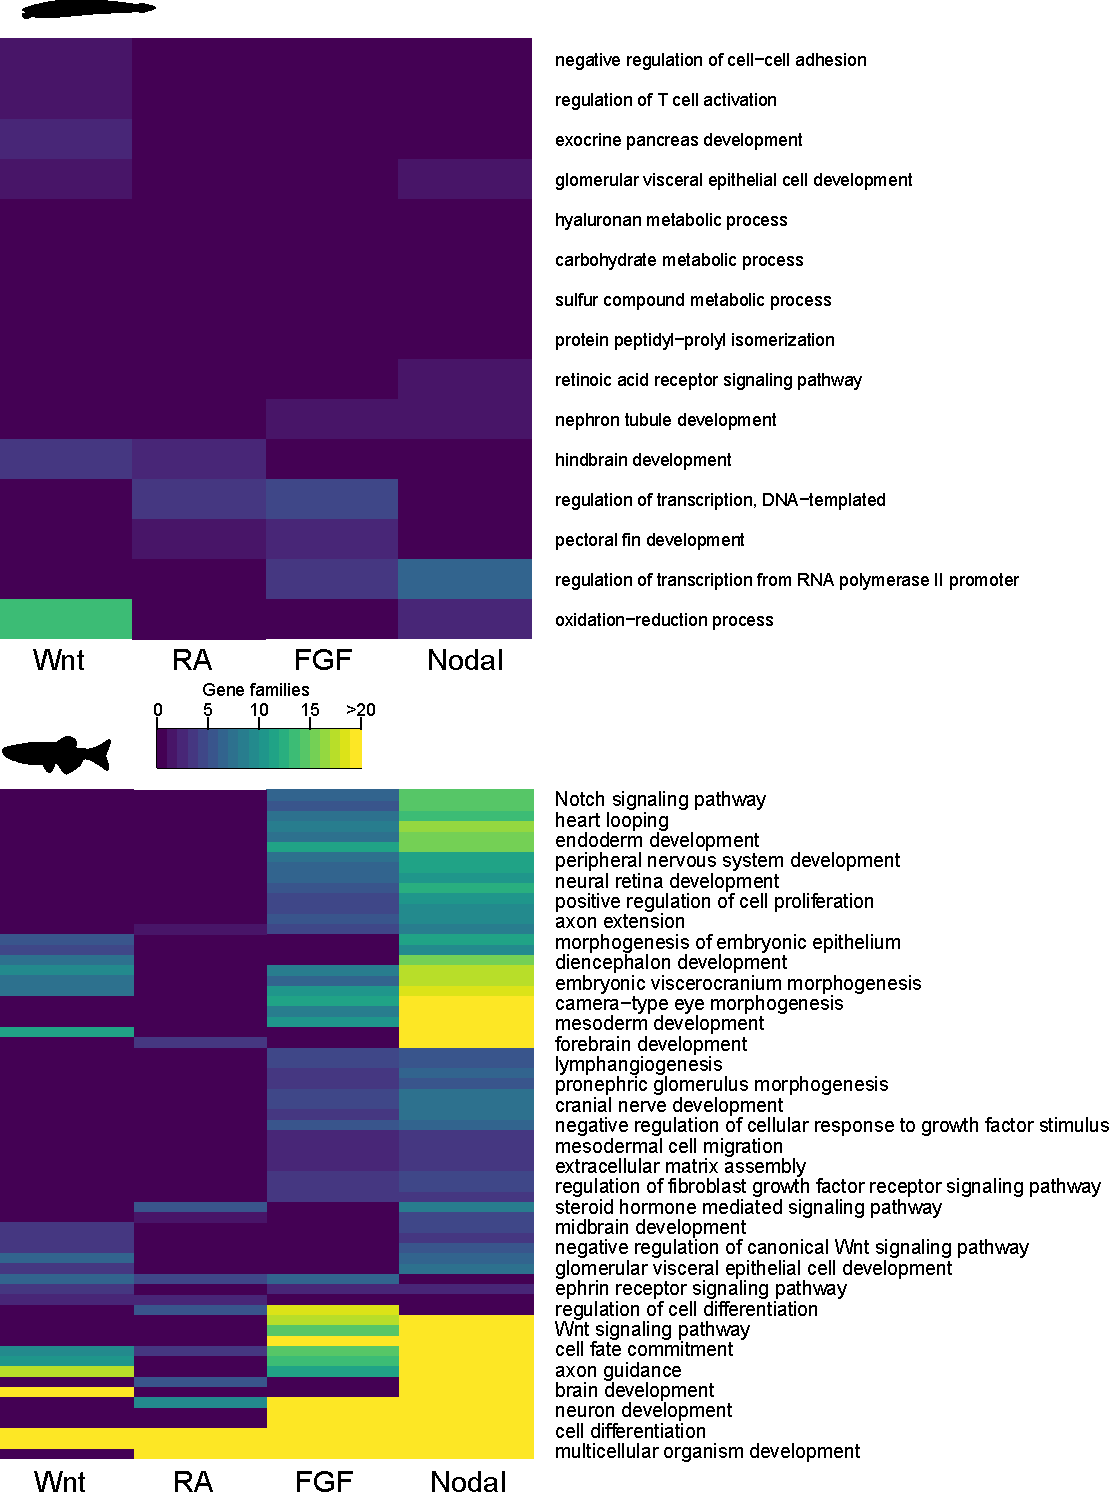
\includegraphics[width=1\textwidth]{Figures/DSG_GOs_fams}
\caption[GO enrichment clustering of DSGs in both species, using families]{GO enrichment clustering of DSGs in both species. The heatmaps show how the different GO terms are clustering based on the number of gene families in amphioxus (top) and in zebrafish (bottom). Modified from \parencite{gil-galvez_gain_2022}.
}
\label{fig:DGS_GOs_fams}
\end{figure} 

 
To shed light on the observed gain of connectivity in vertebrates, we generated connectivity scores for genes regarding the number of treatments to which they respond. Similarly to what we did with DARs connectivity, this score ranges from 1 to 4, representing the number of treatments they responded to. We performed this analysis for genes that responded and were detected only by RNA-seq and for DSGs. We found that, regardless of the list of genes used, ATAC-seq \& RNA-seq (DSGs), or RNA-seq only genes, the connectivity scores were higher in zebrafish in comparison to amphioxus (Figure \ref{fig:Connectivity_genes}). This finding focused on the gene connectivity points towards the same direction as the DAR connectivity (Figure \ref{fig:ATAC_connectivity}). In fact, the greatest difference in connectivity score is observed in the DSG analysis, suggesting that the core of the GRNs, the DSGs, integrate more information through their DARs from different signalling pathways in zebrafish than in amphioxus. Examples of these DSGs are distributed along the genome. For example, the amphioxus \textit{rar} gene is a DSG which responds only to the RA treatment, whereas its orthologous DSG in zebrafish, \textit{rara} responds to both Wnt and RA treatment (Figure \ref{fig:DSG_connec_example}).


\begin{figure}[hp]
\centering
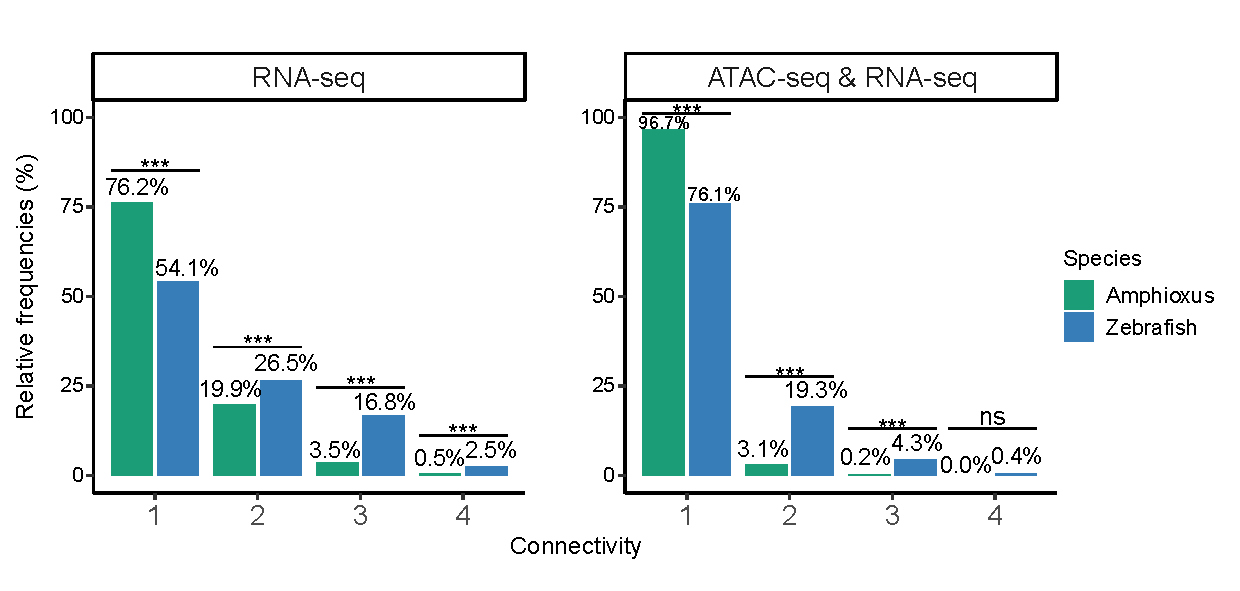
\includegraphics[width=1\textwidth]{Figures/Connectivity_genes}
\caption[Connectivity of genes]{
Barplots showing the connectivity of each gene with the different treatments. This plot shows the percentage of genes that respond to one, two, three or four treatments in zebrafish (blue) and in amphioxus (green). In the left panel, connectivity scores of the genes based only on RNA-seq are represented, while in the right panel, both RNA and ATAC-seq are considered. *P value < 0.05; **P value < 0.01; ***P value < 0.001. Modified from \parencite{gil-galvez_gain_2022}. }
\label{fig:Connectivity_genes}
\end{figure} 


\begin{figure}[hp]
\centering
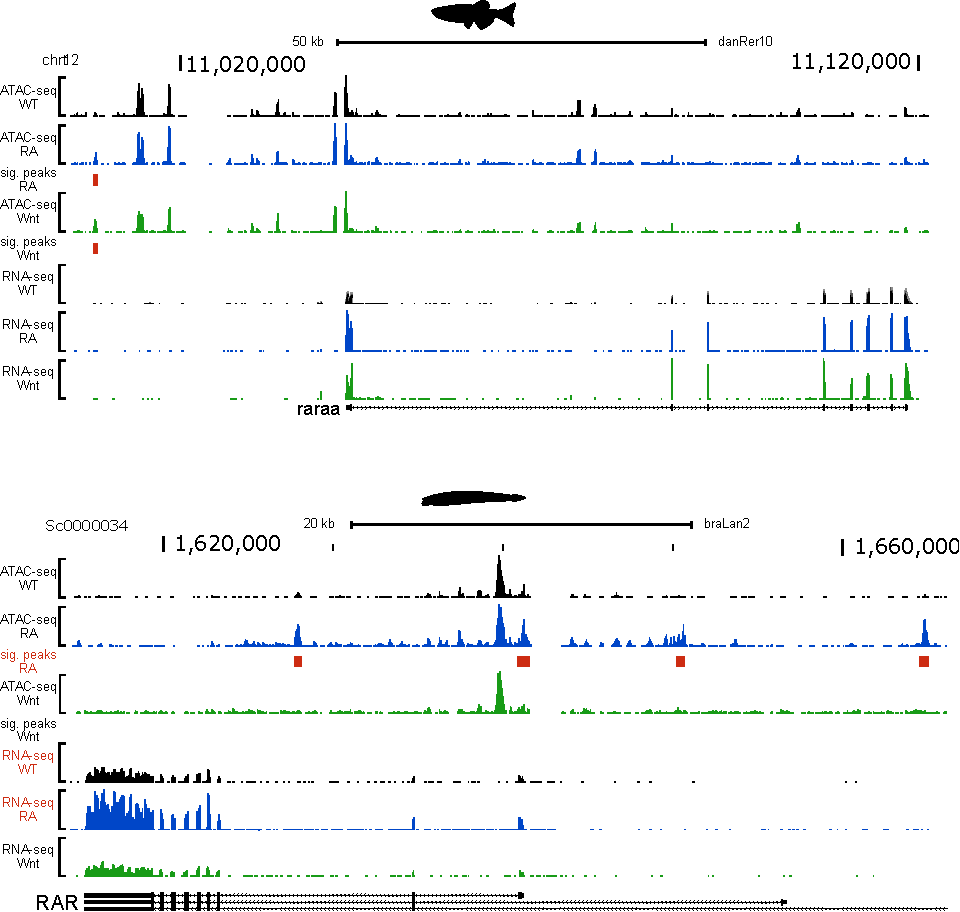
\includegraphics[width=1\textwidth]{Figures/DSG_connec_example}
\caption[Example of connected DSG]{Example of a gene that has gained connectivity in zebrafish. The \textit{rar} gene in amphioxus (bottom) is only responding to RA treatment, whereas in zebrafish (top) is also responding to Wnt treatment. The responsive DARs are marked in red.}
\label{fig:DSG_connec_example}
\end{figure} 




Since WGDs have a great impact on gene regulation, we wondered whether this connectivity gain depended on how many genes were retained after WGD. We found that in zebrafish, the connectivity of RNA-seq responsive genes was greater than in amphioxus genes, regardless of how many copies were retained after WGD (Figure \ref{fig:Connectivity_genes_wgd}). We observed that ohnologs retained in a 1-to-1 manner tended to be less connected compared to those retained in a 1-to-many manner (one copy in amphioxus corresponds to more than two in zebrafish) in the same species. For example, in zebrafish, responsive genes that were maintained in a 1-to-1 fashion and responded to the four treatments represented only 0.4\% of the total of 1-to-1 responsive genes. This percentage increased to 2.1\% when considering the same level of connectivity in genes that were retained in a 1-to-many fashion. We then classified the genes into more specific categories based on the number of copies retained (e.g. 1:1, 1:2, 1:3, and 1:4 or more). We found that the more copies of a gene were retained in vertebrates, the more connectivity tended to have this gene in zebrafish, suggesting that there are some copies of genes that have gained regulatory information with respect to others (Figure \ref{fig:Connectivity_genes_wgd}). 


\begin{figure}[h]
\centering
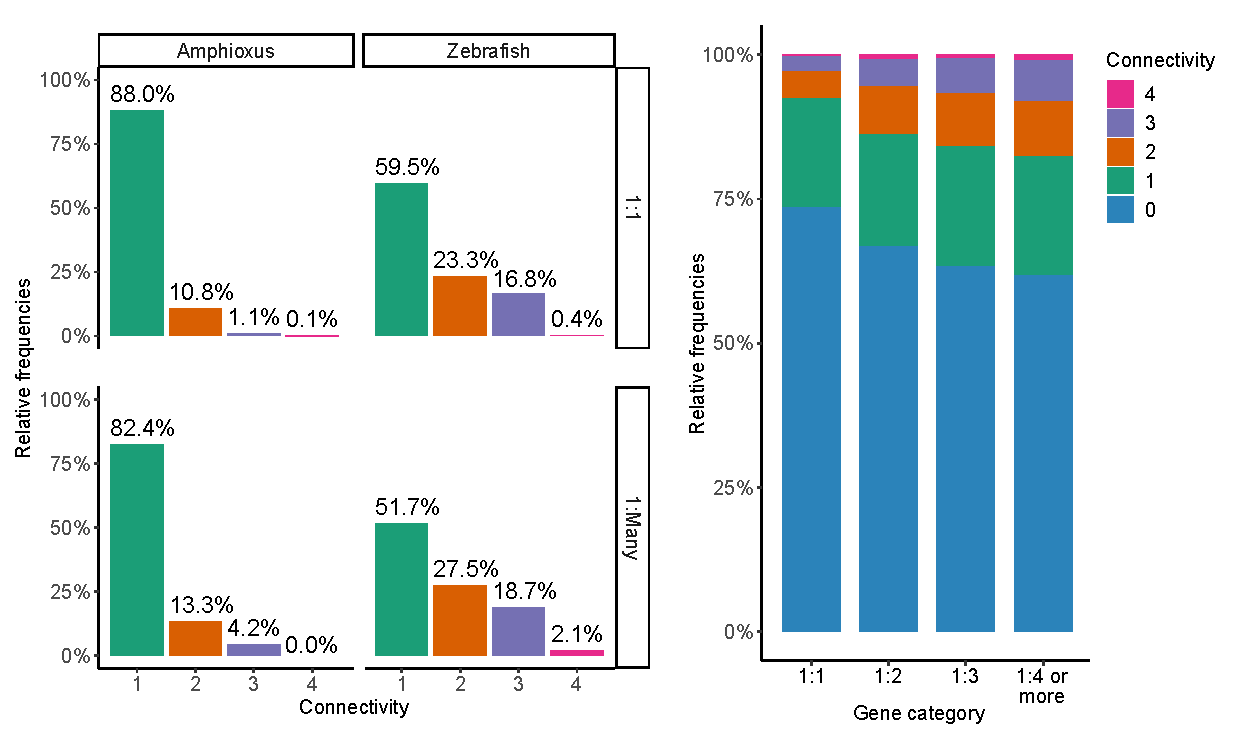
\includegraphics[width=1\textwidth]{Figures/Connectivity_genes_wgd}
\caption[Connectivity of DSGs according to their ohnologs]{
Connectivity of DSGs according to the number of ohnologs in zebrafish. The left bar plots show the connectivity of those genes that retained only one copy (1:1) or many (1:many) in amphioxus and in zebrafish. The right panel shows the connectivity levels of the genes that were retained in one, two, three or four or more than four copies. Modified from \parencite{gil-galvez_gain_2022}. }
\label{fig:Connectivity_genes_wgd}
\end{figure} 

In order to eliminate potential bias due to the selected species, we performed similar experiments in other two species, the vertebrate tetrapod \textit{Xenopus tropicalis}, and a hemichordate invertebrate, \textit{Ptychodera flava}. We treated the embryos of these species at the blastula stage as in our original experiments with the same antagonists of Nodal and FGF pathways (Figure \ref{fig:Connectivity_new_species}) and generated RNA-seq data. We computed the connectivity score in these species, which can only vary between 1 and 2, since only two signalling pathways are treated. We compared these connectivity scores with their equivalent results in zebrafish and amphioxus. These comparisons showed a general increasing trend in connectivity in vertebrates compared to invertebrates. We could then compare the connectivity level of the genes in the four species in a pairwise manner. When comparing amphioxus to \textit{Ptychodera flava}, we did not find statistically significant differences between them (\textit{P} value = 0.545, \(\chi^2\) test), but when we compared the new vertebrate species \textit{X. Tropicalis}, with amphioxus and \textit{P. flava}, we found a significant gain in connectivity (\textit{P} values of 0.048 and 0.006, respectively, \(\chi^2\) test) (Figure \ref{fig:Connectivity_new_species}). Since zebrafish suffered an extra round of WGD compared to \textit{X. Tropicalis}, we could expect a gain in connectivity due to potentially higher GRN complexity. However, although we could observe some differences in the connectivity of zebrafish against \textit{X. Tropicalis}, these differences were not statistically significant (\textit{P} value = 0.196, \(\chi^2\) test). 




\begin{figure}[hp]
\centering
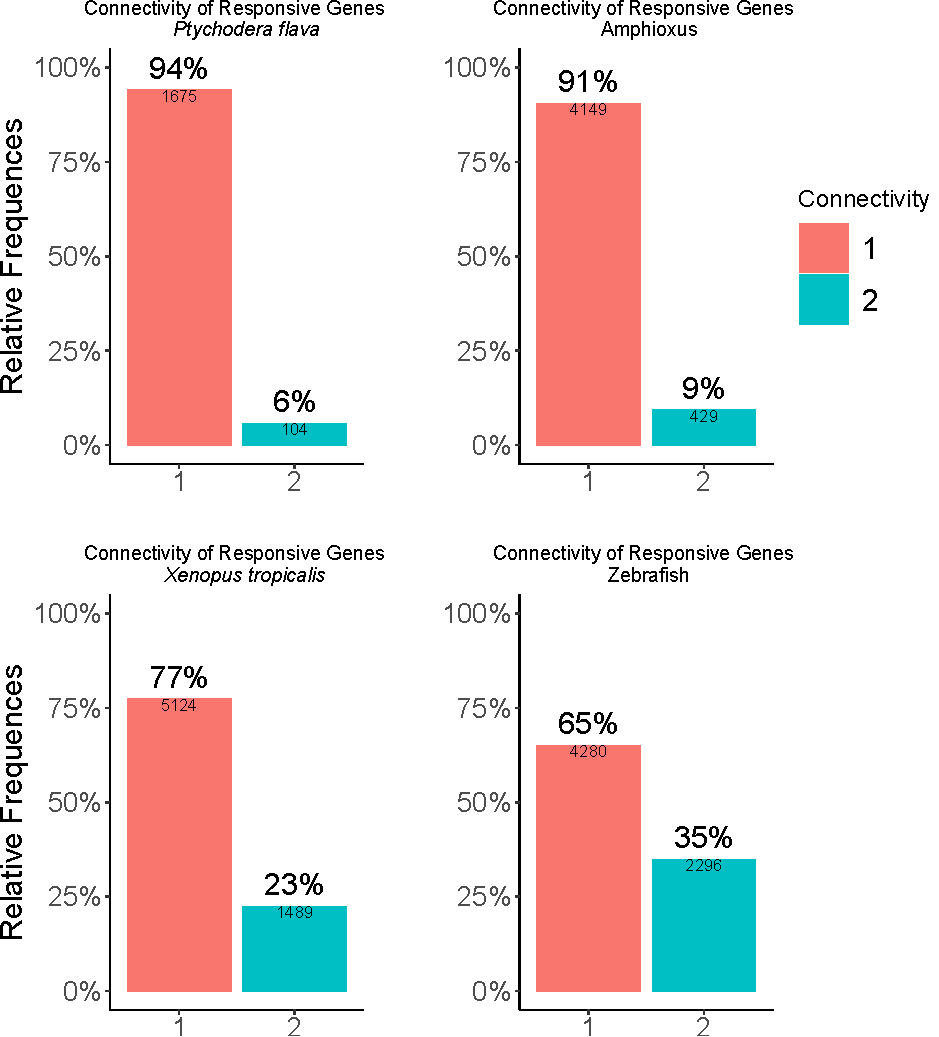
\includegraphics[width=1\textwidth]{Figures/Connectivity_new_species}
\caption[Connectivity of the new species]{Bar plots representing the percentage of genes that respond to one or two treatments in the hemichordate \textit{Ptychodera flava}, amphioxus, \textit{Xenopus tropicalis} and zebrafish. Modified from \parencite{gil-galvez_gain_2022}.}
\label{fig:Connectivity_new_species}
\end{figure} 


According to these observations, we wondered about the cause behind this gain of connectivity in vertebrate genes. Did the genes acquire more CREs responding to different pathways, or the existing CREs gained new TFBSs in their sequence? Some of our observations supported the former (Figure \ref{fig:DSG_connec_example}). To address this question, we compared the TFBSs of the unique seven CREs conserved between vertebrates and invertebrates \parencite{royo_transphyletic_2011}. We compared the TFBS scores (how good is the match between the genomic sequence and the TFBS recognition) of these elements in zebrafish and amphioxus, but we could not find a significant difference between them (Figure \ref{fig:Ultraconserved_TFBS}). To investigate whether any specific TF family gained binding in these regions in zebrafish, we aggregated the TFBSs based on their TF family, and we could not find any specific gain (Figure \ref{fig:Ultraconserved_TFBS_families}). Next, we classified DARs according to their evolutionary age and compared their connectivity. We found that the later the DAR arose, the more connected they are (Figure \ref{fig:DARs_connect_evolutionary_age}). 
All these findings, together with the higher number of regulatory elements in zebrafish than in amphioxus observed in previous works \parencite{marletaz_amphioxus_2018}, point towards an increase of regulatory complexity due to a gain in regulatory elements after WGD events in vertebrates.


\begin{figure}[hp]
\centering
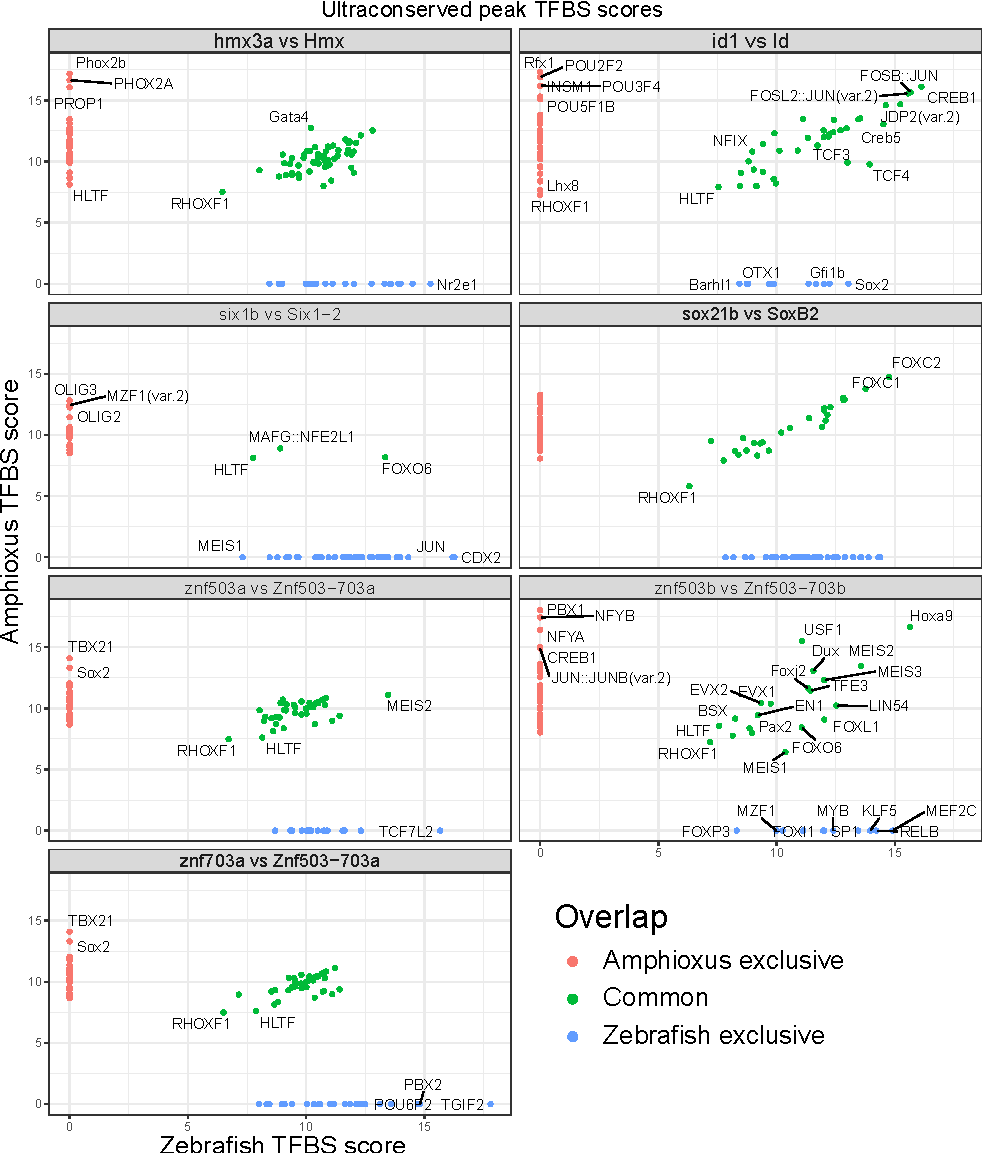
\includegraphics[width=1\textwidth]{Figures/Ultraconserved_TFBS}
\caption[Ultraconserved TFBS]{Scores of TFBS found in ancestral enhancers. Seven regulatory regions that showed conservation between amphioxus and vertebrates were scanned using the JASPAR Core database. Each panel represents an ancient enhancer, with the score of TFs found in the zebrafish sequence represented in the X-axis and the amphioxus score in the Y-axis. TFs found in both species are represented in green, whereas those found only in zebrafish or amphioxus are represented in blue and red, respectively. Modified from \parencite{gil-galvez_gain_2022}.}
\label{fig:Ultraconserved_TFBS}
\end{figure} 


\begin{figure}[hp]
\centering
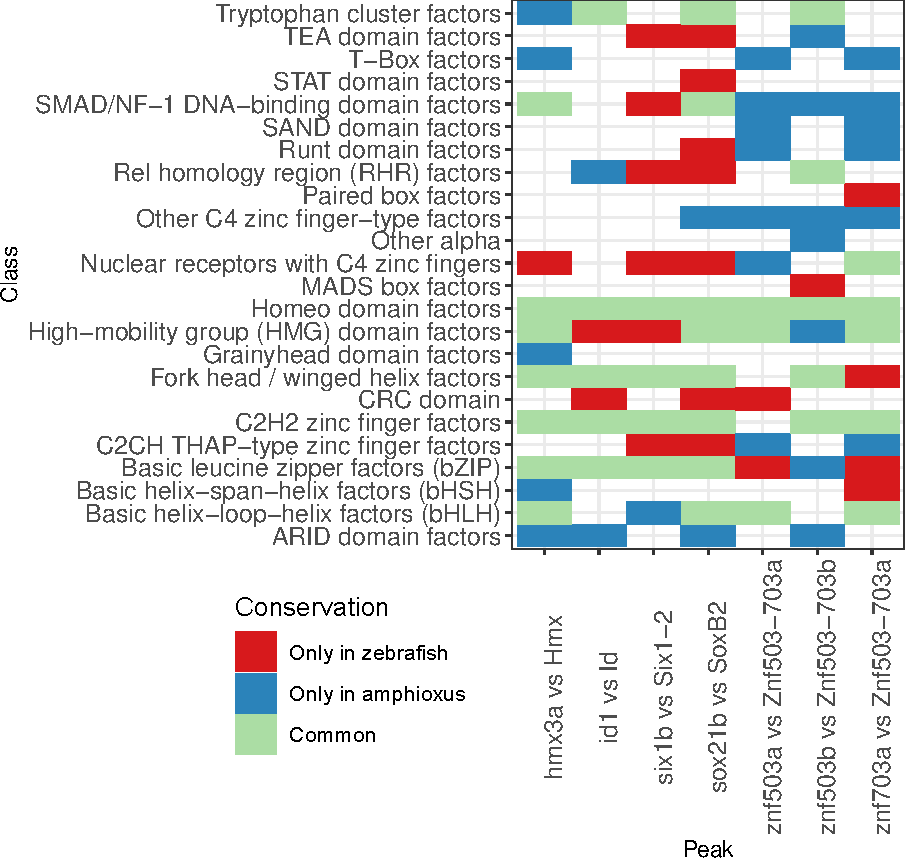
\includegraphics[width=1\textwidth]{Figures/Ultraconserved_TFBS_families}
\caption[Ultraconserved TFBS families]{Families of TFs found in the ancient enhancers. Seven ancient enhancers are represented in the X-axis, and TF families in the Y-axis. TF families found only in zebrafish, only in amphioxus and in both species are represented in red, blue and green, respectively. Modified from \parencite{gil-galvez_gain_2022}.}
\label{fig:Ultraconserved_TFBS_families}
\end{figure} 


\begin{figure}[h]
\centering
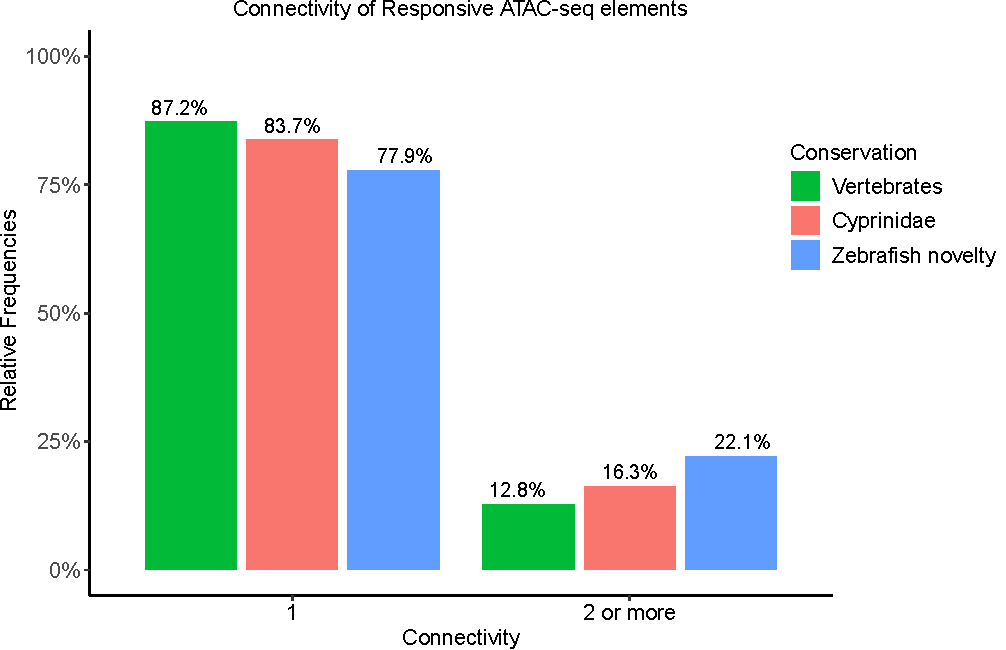
\includegraphics[width=1\textwidth]{Figures/DARs_connect_evolutionary_age}
\caption[Newer DARs show more connectivity than older ones]{Bar plot showing the connectivity of three different groups of DARs, classified by their evolutionary age. From ancient to newer, there are represented DARs that are conserved in vertebrates, in Cyprinidae and those that are zebrafish novelties. The connectivity is inversely proportional to the evolutionary age. Modified from \parencite{gil-galvez_gain_2022}.}
\label{fig:DARs_connect_evolutionary_age}
\end{figure} 

In order to understand how the gain of connectivity influences the development of the vertebrate body plan, we investigated the tissues that expressed genes with more connectivity. To do this, we used published single-cell RNA-seq (scRNA-seq) experiments performed in zebrafish embryos \parencite{farnsworth_single-cell_2020}. Intersecting this scRNA-seq atlas with the list of genes that gain connectivity in vertebrates, we could analyze their expression pattern during development in a quantitative manner. We selected tissues taking into account their evolutionary age: a group of tissues that are considered vertebrate novelties like placodes, neural crest, or retina, and other group of tissues like muscle, intestine, or blood, which are considered to be ancestral to all chordates. We then estimated the number of cells in each tissue that expressed highly connected genes or lowly connected genes (Figure \ref{fig:SingleCell_connectivity}).  We found that these genes were evenly enriched in ancient tissues, and we could not find any statistically significant differences in this enrichment. On the contrary, in novel tissues, we found that highly connected genes were more represented than lowly connected genes. In addition, we computed the ratio between highly and lowly connected genes for each tissue and found that, in tissues considered as vertebrate novelties, this ratio tended to be higher than in ancient tissues (Figure \ref{fig:SingleCell_connectivity_ratio}).



\begin{figure}[h]
\centering
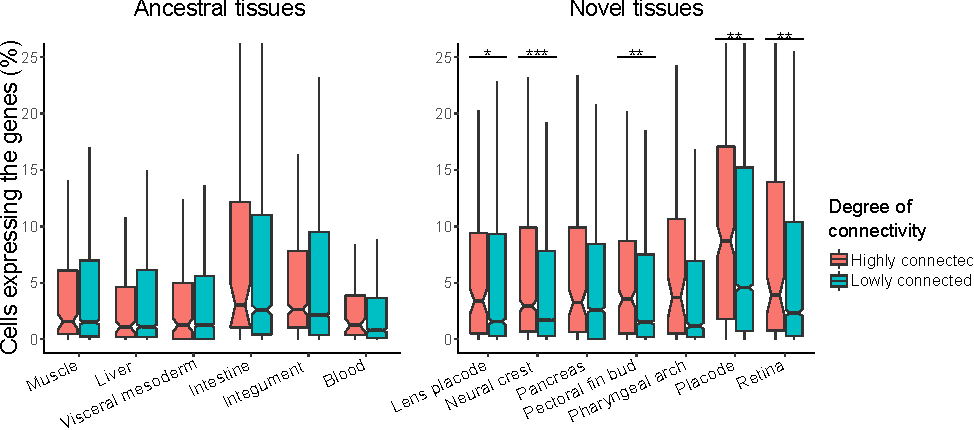
\includegraphics[width=1\textwidth]{Figures/SingleCell_connectivity}
\caption[Single-cell RNA-seq connectivity enrichment ]{Expression of connected genes in different tissues. Boxplots represent the percentage of cells that express highly connected genes (connectivity score $\geq $ 3, pink colour) or lowly connected genes (connectivity score = 1). Expression data comes from scRNA-seq experiments \parencite{farnsworth_single-cell_2020}. The left panel corresponds to tissues considered ancestral between cephalochordates and vertebrates, whereas in the right panel, tissues that are vertebrate novelties are represented. Boxes represent the first, second and third quartiles, and the lines represent the range.  Notations: * P value < 0.05; ** P value < 0.01; *** P value < 0.001. Modified from \parencite{gil-galvez_gain_2022}.}
\label{fig:SingleCell_connectivity}
\end{figure} 




\begin{figure}[h]
\centering
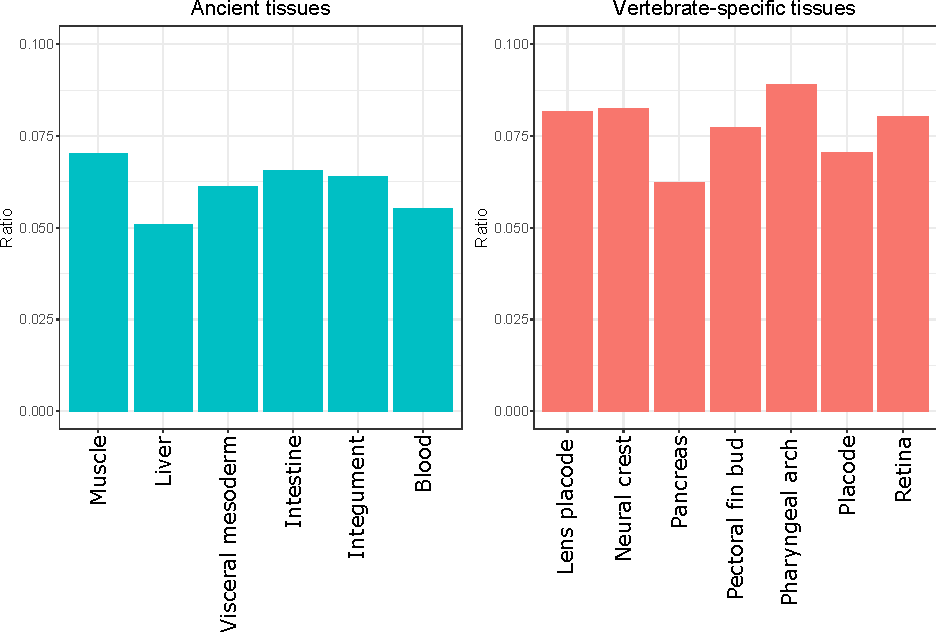
\includegraphics[width=1\textwidth]{Figures/SingleCell_connectivity_ratio}
\caption[Single-cell RNA-seq connectivity ratios]{Barplots represent the ratio between the number of highly connected genes (connectivity score $\geq$ 3) and lowly connected genes (connectivity score = 1) that are expressed in ancient tissues (left panel) and tissues that are vertebrate novelties (right panel). Modified from \parencite{gil-galvez_gain_2022}.}
\label{fig:SingleCell_connectivity_ratio}
\end{figure} 


To better visualise the connections between the different signalling pathways in amphioxus and zebrafish, we used Cytoscape \parencite{shannon_cytoscape_2003}. Using this tool, we generated interaction networks between the four different signalling pathways and DSGs. This powerful visualisation showed great differences in the connectivity between amphioxus and zebrafish (Figure \ref{fig:Cytoscape_connectivity}). We found that in amphioxus, only a few DSGs responded to more than one signalling pathway, whereas, in zebrafish, this was a more common phenomenon, which helps to visualize the great gain of gene regulatory connectivity in zebrafish genes compared to amphioxus.

Together these results demonstrate how signalling pathways have been rewired in the transition from chordates to vertebrates in order to generate the necessary tissue complexity that vertebrate morphological novelties require. The manipulation of different signalling pathways in zebrafish and amphioxus has revealed that, although the responses and the effectors are conserved between species, the interactions of these signalling pathways have evolved during the invertebrate-to-vertebrate transition. Genes and CREs tend to integrate more regulatory information in their regulatory regions in the vertebrate lineage. This gain of interconnectivity was probably provided by the vertebrate WGDs, which allowed the emergence of new developmental copies of key genes that integrate this novel information. These regulatory hubs have probably contributed to the emergence of vertebrate morphological novelties.


\begin{figure}[h]
\centering
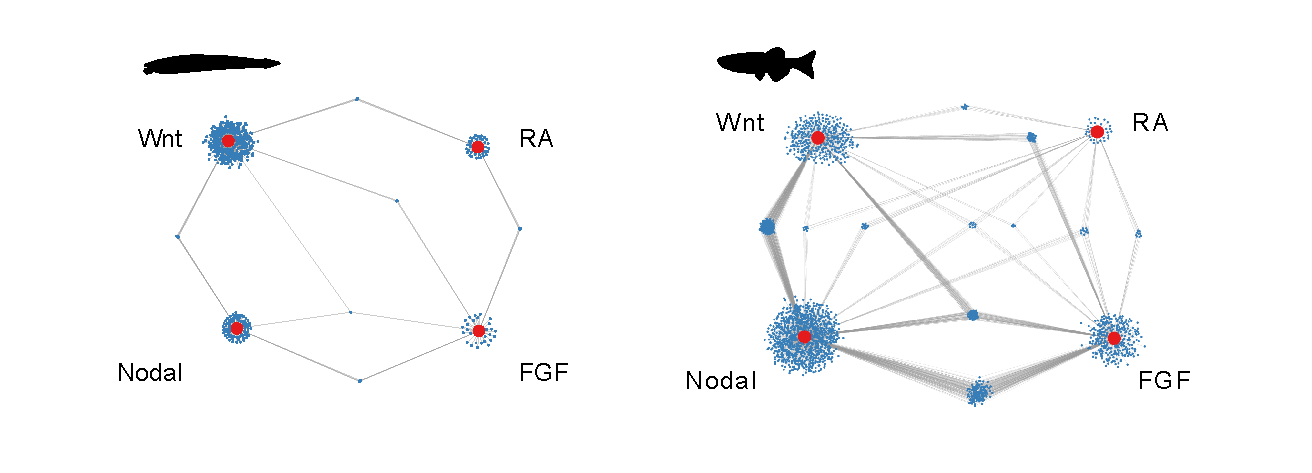
\includegraphics[width=1\textwidth]{Figures/Cytoscape_connectivity}
\caption[Cytoscape connectivity]{Connectivity network of the altered signalling pathways in amphioxus (left) and zebrafish (right). The graph has been built using Cytoscape software. Each red node represents one of the four different signalling pathways, and each DSG is a blue dot. The edges of the network (grey lines) represent the responsiveness of each DSG with the corresponding signalling pathway. Modified from \parencite{gil-galvez_gain_2022}.}
\label{fig:Cytoscape_connectivity}
\end{figure} 


